\documentclass[12pt]{article}

%%%% packages and definitions (optional)
\usepackage{graphicx} % allows inclusion of graphics
\usepackage{graphics}
\usepackage{placeins}
\usepackage{booktabs} % nice rules (thick lines) for tables
\usepackage{microtype} % improves typography for PDF
\usepackage{xspace}
\usepackage[hidelinks]{hyperref}
\usepackage{xspace}
\usepackage{hhline}


\usepackage{pgfgantt}
\usepackage{rotating}
\usepackage[graphicx]{realboxes}
\usepackage{lscape}
\usepackage[margin=0.5in,landscape]{geometry}


\def\pgfcalendarweekdayletter#1{%  
 \ifcase#1M\or Tu\or W\or Tr\or F\or Sa\or Su\fi%  
}  
\usepackage{amsmath}

\usepackage{tabularx}
\newcolumntype{b}{>{\hsize=1.0\hsize}X}
\newcolumntype{s}{>{\hsize=.5\hsize}X}
\newcolumntype{m}{>{\hsize=.75\hsize}X}

\newcommand{\SN}{S$_N$}
\renewcommand{\vec}[1]{\bm{#1}} %vector is bold italic
\newcommand{\vd}{\bm{\cdot}} % slightly bold vector dot
\newcommand{\grad}{\vec{\nabla}} % gradient
\newcommand{\ud}{\mathop{}\!\mathrm{d}} % upright derivative symbol
\newcommand{\Cyclus}{\textsc{Cyclus}\xspace}%
\graphicspath{ {images/} }
\usepackage[affil-it]{authblk}
\usepackage[numbers]{natbib}
\usepackage{notoccite}
\usepackage{tikz}
\usetikzlibrary{positioning, arrows, decorations, shapes }
\usepackage{cleveref}

\usepackage{datatool}
\usepackage[acronym,toc]{glossaries}
\include{acros}
	
\makeglossaries

\title{Probabilistic Risk Assessment of Mined Nuclear Spent Fuel Repositories }
\author{Jin Whan Bae}
\affil{Dept. of Nuclear, Plasma, and Radiological Engineering, University of Illinois at Urbana-Champaign
		  Urbana, IL}
\date{}                     %% if you don't need date to appear
\setcounter{Maxaffil}{0}
\renewcommand\Affilfont{\itshape\small}
%%%%%%%%%%%%%%actual words%%%%%%%%%%%%%%%%%%%%%%%%%%%%%%%%%%%%%%%%%%%%%%%%%%%%5


\begin{document}
\maketitle

\section{Abstract}
\gls{UNF} repositories, given the high decay heat and radioactivity
of \glspl{UNF}, requires careful engineering. The current plan is
to design a repository that would contain the material for one million years.
Considering various events (failures) can occur in that time range,
the \gls{UNF} repository proposes an interesting subject for
\gls{PRA}. In this report, the model repository design is after the 
\gls{YMR}, which is a mined repository in volcanic tuff.
Ultimate failure status can be defined in various ways, depending on the
extent of leakage during the one million years (leakage from canister
\textasciitilde exposure to nearest population).
A definitive exposure of failure criteria must be defined,
in order for a reasonable analysis.  

Given the expansive
time range, very little real data is available, which makes
most of the probability values a Bayesian, a `degree-of-confidence' value.
Other data can be derived from scientific data, such as 
corrosion and precipitation in the area, but would have to be extrapolated
with assumptions for the given time range.

The failure scenario would begin from the canister's arrival at the
site, namely, from the repackaging facility. The repackaging facility
would take out the individual assemblies from the transportation cask
and emplace the assemblies in a storage cask. There, the storage cask
would be moved to the repository to sit for a million years. 
Given the successful emplacement of the fuel canister, the canister
must corrode, or break, in order to expose the radioactive materials
inside. The exposed radioactive materials would be transported, through
various methods (person carrying it out, precipitation flow etc.)
to affect the population, causing the system to fail.


\section{Goal}
The goal of this project is to create a simplistic case study of the
\gls{YMR} with RISKMAN. Various aspects of the repository
will be modeled in different ways, from empirical failure point probability data,
distributions with uncertainty, and human failure models.

\section{Schedule}
\noindent\resizebox{\textwidth}{!}{
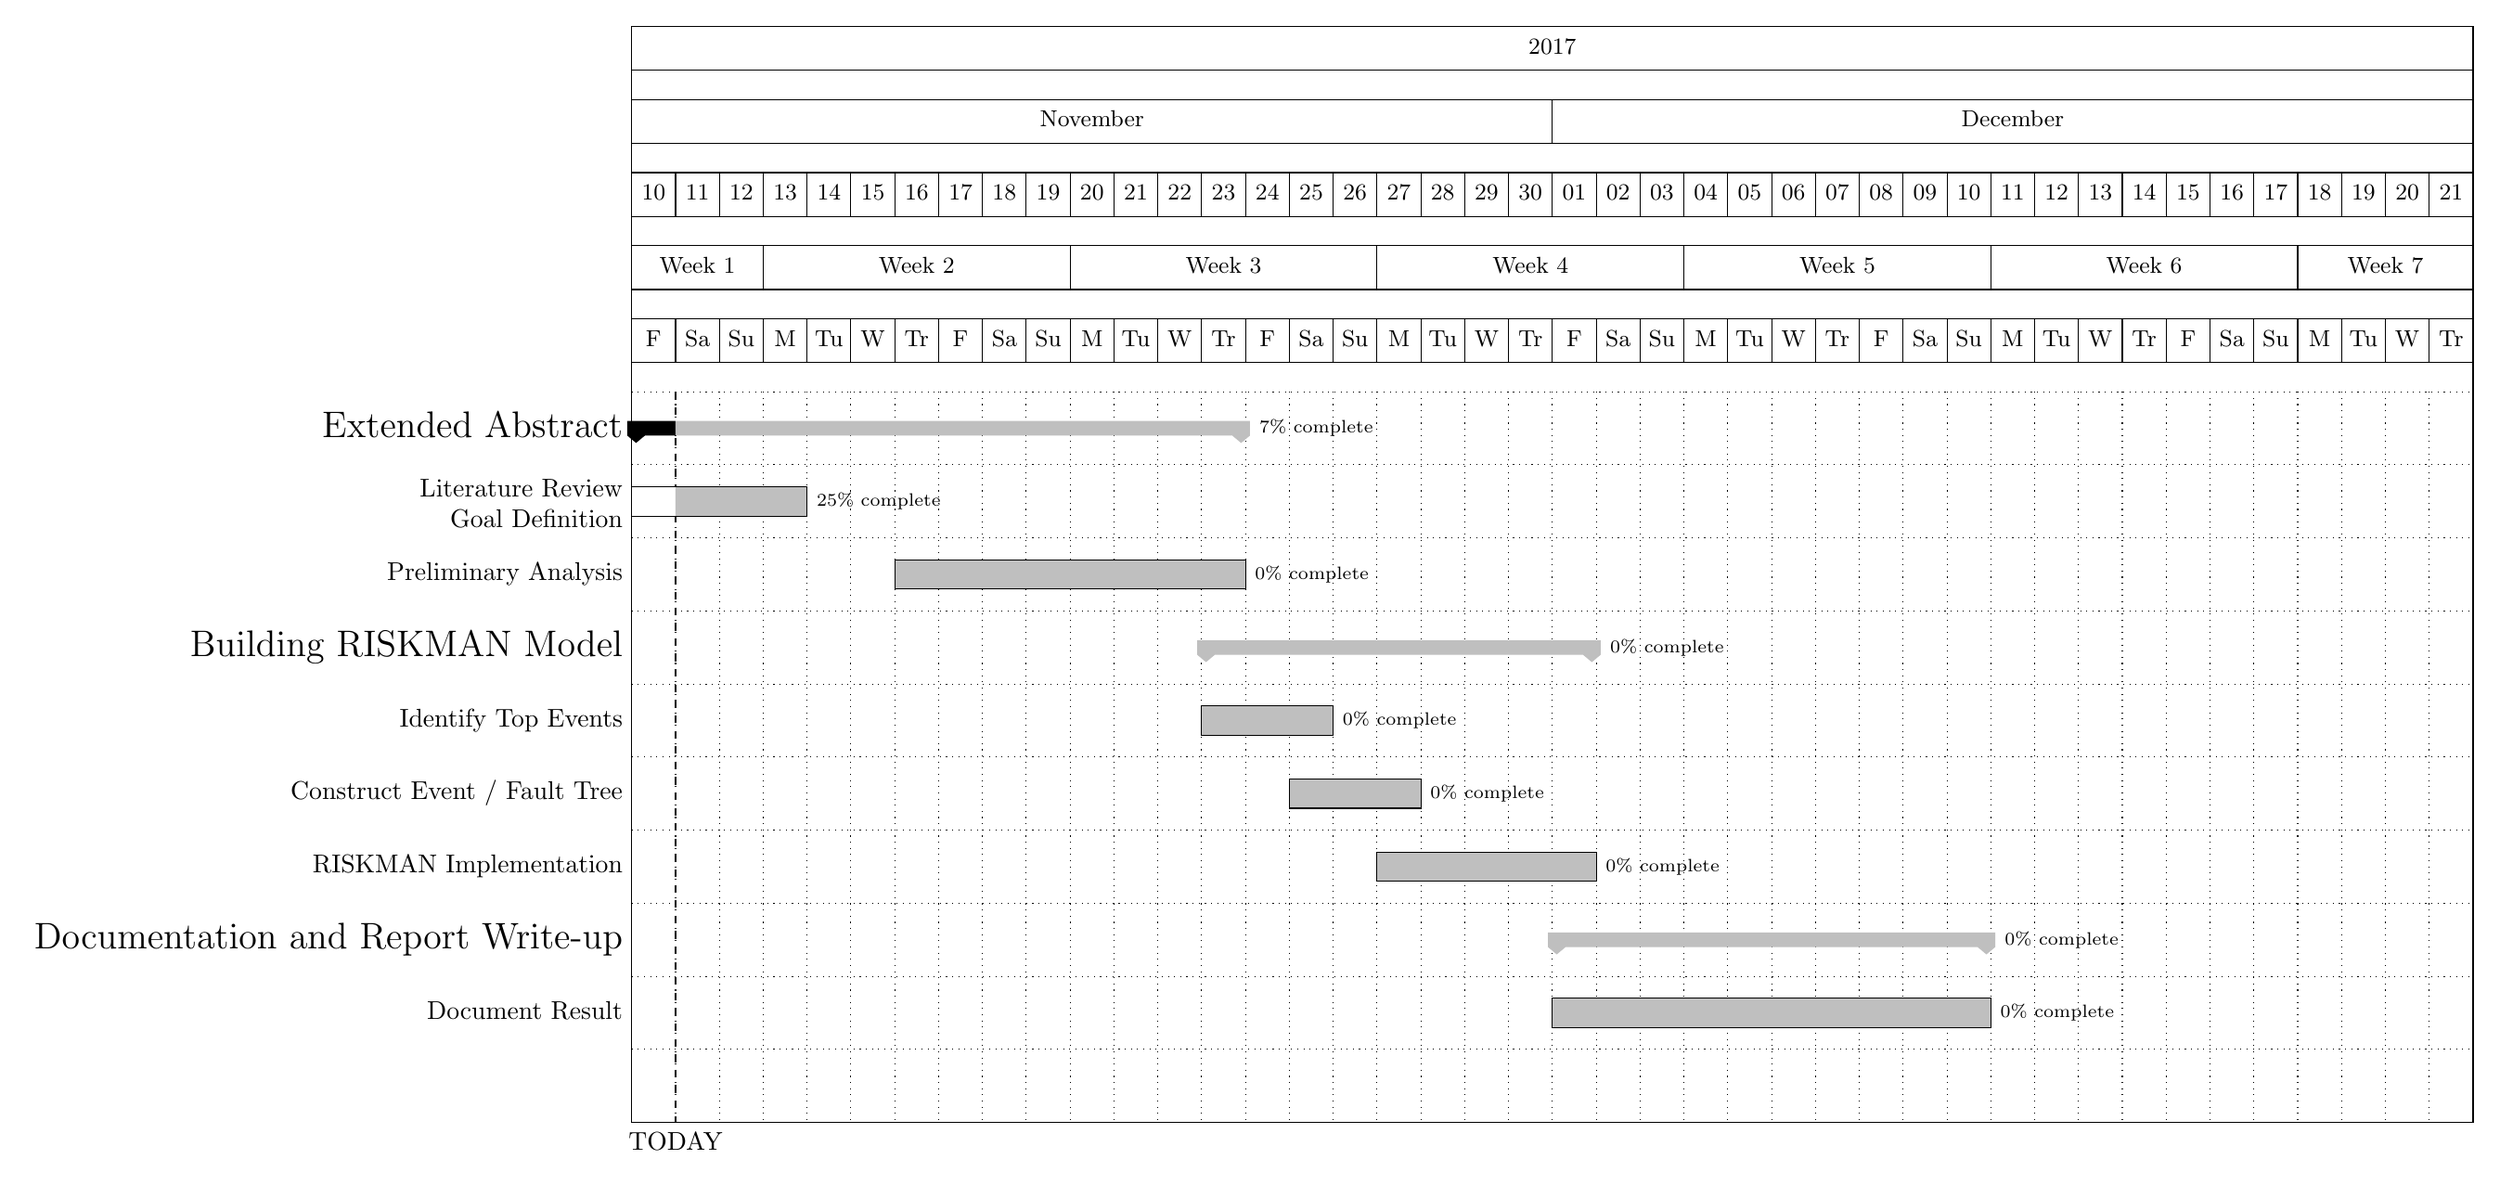
\begin{tikzpicture}[x=.5cm, y=1cm]
\begin{ganttchart}[
    hgrid,
    vgrid,
    group label font=\Large,
    progress=today,
    today=2017-11-10,
    x unit=6mm,
    newline shortcut=true,
    bar label node/.append style={align=right},
    time slot format=isodate
    ]{2017-11-10}{2017-12-21}
    \gantttitlecalendar{year, month=name, day, week=1, weekday=letter} \\
    
    \ganttgroup{Extended Abstract}{2017-11-10}{2017-11-23} \\
    \ganttbar{Literature Review \ganttalignnewline Goal Definition}{2017-11-10}{2017-11-13} \\
    \ganttbar{Preliminary Analysis}{2017-11-16}{2017-11-23} \\

    
    \ganttgroup{Building RISKMAN Model}{2017-11-23}{2017-12-01} \\
    \ganttbar{Identify Top Events}{2017-11-23}{2017-11-25}\\
    \ganttbar{Construct Event / Fault Tree}{2017-11-25}{2017-11-27} \\
    \ganttbar{RISKMAN Implementation}{2017-11-27}{2017-12-01} \\

    \ganttgroup{Documentation and Report Write-up}{2017-12-01}{2017-12-10}\\
    \ganttbar{Document Result}{2017-12-01}{2017-12-10} \\
    
    

    
\end{ganttchart}
\end{tikzpicture}
}


\section{Background}
\gls{YMR} has been studied thoroughly in hopes of finally
disposing the U.S. \gls{UNF} inventory. However, considering
that it is a large project involving highly radioactive material,
careful planning and analyses must be done. The reference design
is taken from various sources \cite{u.s._department_of_energy_office_of_civilian_radioactive_waste_management_national_2008, wilson_total-system_1994, rechard_evolution_2014}.
The RISKMAN model will attempt to capture various factors in the design.


\section{Literature Review}
System designs of the \gls{YMR} are listed extensively in literature \cite{u.s._department_of_energy_office_of_civilian_radioactive_waste_management_national_2008, wilson_total-system_1994, rechard_evolution_2014}, and contain multiple
iterations on the design. The basic design is as follows: the spent fuel assemblies
are repackaged in the waste package canister, and then placed underground,
underneath a drip shield. The canisters will remain there for up to millions of years,
surrounded by volcanic tuff.

Some prominent risk factors have also been identified. Volcanic hazards \cite{ho_risk_1992, smith_area_1990}
have been identified to be a long-term issue. Groundwater movement and transport of 
radioactive isotopes are another issue, in the case of canister breach \cite{robison_ground-water_1984, quade_fossil_1995}.  Canister reliability is another
identified risk factor \cite{whipple_can_1996, rutqvist_analysis_2003}.

Different aspects of risk analysis for nuclear waste repositories are published.
For systems where the future is hardly predictable, bayesian network analyses are 
suggested in \cite{lee_application_2006}. A method for sensitivity analysis
to rank important parameters are suggested in \cite{mohanty_cdf_2001}.


\section{Method}

From the literature review, a crude diagram of the \gls{YMR} system is drawn.
From the diagram, important subsystems are identified, with possible initiating
events that cause them to fail. The subsystems are then linked upon their dependence.
The initiating events and the related event trees are developed, along with the
fault tree of the events, if applicable. The probability of basic events or components
then would be modeled
appropriately, using various methods like point estimate or distributions.
The constructed system reliability analysis model then would be implemented to
RISKMAN, in order to calculate the reliability of the system and identify
important components or human factors to consider.











\bibliographystyle{unsrtnat}
\bibliography{bibliography}


\end{document}
\grid
